\chapter{Technical Approach}

\section{Background}
\subsection{Data-flow Analysis}
In compiler theory, data-flow analysis is a technique for gathering information about the possible set of values calculated at various points in a computer program. The basis for performing data-flow analysis is control flow graph (CFG), which is used to determine those parts of the program to which a particular value assigned to a variable might propagate. In our particular case, we used reaching-definition for each instruction to represent the data flow information. Two techniques applied for performing reaching-definition analysis are \textit{Liveness Analysis} and \textit{Reaching-Def Analysis}.

%CFG and ICFG
Control Flow Graph (CFG) is a graph representation of all the paths that a computer program might be traversed through during its execution. In a control flow graph, each node represents a basic block - a sequencial piece of a program that does not include jumps or jump targets, while the directed edges represent jumps in the program. Figure 2.1 is the complete control flow graph constructed for an example function t3f1. Each circle represents a basic block (first number in the circle denotes its line number), and the black edges represent the possible jumps that the program can take during execution. It is worth noting that the while loop in t3f1 includes a condition check at line 4, which can be reached from either line 4 (before loop starts) or from line 13 (after last instruction in the loop is finished). Therefore in the CFG there are two nodes representing line 5, with one coming from line 4 and another coming from line 13.

\begin{figure}
\begin{minipage}{\textwidth}
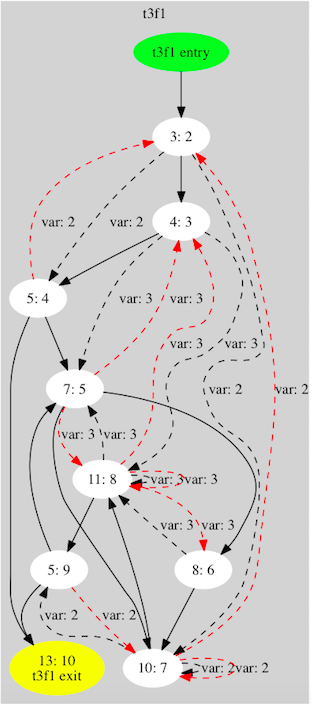
\includegraphics[width=0.6\textwidth]{figures/CFG.png}
\caption{Control Flow Graph for Function t3f1}
\label{CFG}
\end{minipage}
\end{figure}

\lstset{language=PHP}
\begin{minipage}{0.5\textwidth}
\begin{lstlisting}[frame=single]
<?php
function t3f1($c, $d) {
  $a = 0;
  $b = 0;
  while($a <= 5)
  {
    if ($b > 5) {
      $b = 5;
    }
    $a = $a + 1;
    $b = $b + 2;
  }
}
?>
\end{lstlisting}
\end{minipage}
\newline

%liveness analysis and reaching-def analysis
As one of the two techniques used for performing reaching-definition analysis, liveness analysis is to calculate, at instruction level, the variables that may be potentially read before their next write, that is, the variables that are live at the exit from each program point. In the given example, variable b is first defined at line 4; it is also defined at line 8 and 11 in the main loop. Therefore, var b is said to be "alive" from line 4 to line 8, and from line 11 back to line 8. Given liveness analysis output, def-use chains can be constructed for each variable. The DU chain represents the exact places where a variable definition is later used in other instructions. The DU chains in t3f1 are shown as black dotted edges in Figure 2.1.

To the contrary of liveness analysis, reaching-def analysis calculates the possible definition instructions for a given use variable. Reaching-def analysis helps generate use-def chains for each variable used in a program. The UD chains for variables in t3f1 are shown as red dotted edges in Figure 2.1.

\subsection{HipHop Bytecode}
\blindtext

\section{Inter-procedural CFG Construction}
Usually during static analysis, an intra-procedural CFG is constructed for each individual function before all intra-procedural CFGs are combined into one inter-procedural CFG (ICFG) that represents the control flow for the entire program. ICFG is a combination of all individual functions and a function call graph (CG), which is a graph representation of function dependencies in a program, in which functions are represented as nodes and function invokations are represented as directed edges. Since one variable defined/used in any function can be used/defined in other functions, extra work needs to be done in order to expand a variable's DU and UD chains in ICFG. Algorithm 1 shows the construction of DU and UD chains in ICFG given individual CFGs and CG.

\algdef{SE}[UNTIL]{Until}{EndUntil}[1]{\algorithmicuntil\ #1\ \algorithmicrepeat}{\algorithmicend\ \algorithmicuntil}%
\begin{algorithm}
\caption{Dataflow Expansion in ICFG}
\begin{algorithmic}[1]
\Require 
  \State $CG$: call graph of the application program; 
  \State $CFGS$: CFGs for all functions in the program

\Comment{main}
\Procedure{Dataflow Expansion}{}
\State{$visited$ $\gets$ $\emptyset$}
\For{Each $CFG$ in $CFGS$}
  \For{Each instruction $I$ in $CFG$}
    \If{$I$ has KILL variable $kv$}
      \State\Call{completeDefUse}{$CFG$, $I$, $kv$, $visited$}
    \EndIf
  \EndFor
\EndFor

\State{$visited$ $\gets$ $\emptyset$}

\For{Each $CFG$ in $CFGS$}
  \For{Each instruction $I$ in $CFG$}
    \If{$I$ has GEN variable $gv$}
      \State\Call{completeUseDef}{$CFG$, $I$, $gv$, $visited$}
    \EndIf
  \EndFor
\EndFor
\EndProcedure

\algstore{alg1}
\end{algorithmic}
\end{algorithm}

\begin{algorithm}
\begin{algorithmic}[1]
\algrestore{alg1}
\Function{completeDefUse}{$cfg$, $instr$, $var$, $visited$}
  \If{$instr$ in $visited$}
    \State\Return{$instr.duchain$}
  \EndIf
  \For{Each Use $use$ in $instr.duchain$}
    \If{$use$ is a function call site}
      \State Get the callee function $targetfunction$
      \State Get the function parameter $targetvar$ in $targetfunction$ that corresponds to $use.var$
      \State Get the instruction $targetInstr$ that initiates $targetvar$ in $targetfunction$
      \State $newuses$ $\gets$ \Call{completeDefUse}{$targetfunction.CFG$, $targetInstr$, $targetvar$, $visited$}
      \State $instr.duchain$ $\gets$ ($instr.duchain$ - $use$) $\cup$ $newuses$
    \EndIf
  \EndFor
  \State $visited$ $\gets$ $visited$ $\cup$ $instr$
  \State\Return{$instr.duchain$}
\EndFunction
\algstore{alg1}
\end{algorithmic}
\end{algorithm}

\begin{algorithm}
\begin{algorithmic}[1]
\algrestore{alg1}
\Function{completeUseDef}{cfg, instr, var, visited}
  \If{$instr$ in $visited$}
    \State\Return{$instr.udchain$}
  \EndIf
  \For{Each Def $def$ in $instr.udchain$}
    \If{$def$ is a function entry site}
      \State Get all the functions $callerfuncs$ that calls current function
      \For{Each function $callerfunc$ in $callerfuncs$}
        \State Get the function parameter $sourcevar$ in $callerfunc$ that corresponds to $def.var$
        \State Get the instruction $sourceInstr$ in $callerfunc$ that passes $sourcevar$ to callee stack
        \State $newdefs$ $\gets$ \Call{completeUseDef}{$callerfunc.CFG$, $sourceInstr$, $sourcevar$, $visited$}
        \State $instr.udchain$ $\gets$ ($instr.udchain$ - $def$) $\cup$ $newdefs$
      \EndFor
    \EndIf
  \EndFor
  \State $visited$ $\gets$ $visited$ $\cup$ $instr$
  \State\Return{$instr.duchain$}
\EndFunction
\end{algorithmic}
\end{algorithm}

\section{Testcase Generation Algorithm}

\subsection{Precise String Analysis for Input Generation}
Typically, users interact with a web application through a user interface (e.g., web page) that allows them to enter input data (e.g., into a form) and submit such data to the web application via HTTP request. The data that users enter are mostly in string literal forms (e.g., name, address, email, etc). Therefore, generating appropriate string inputs automatically during penetration testing is of our particular interest.

The most direct and effective approach for generating test string literal inputs is to check what values the input variable is compared with during input validation in the application backend. Usually after the application receives a request from the client side, it will compare each input field against some specific values or regular expressions, in order to check if the value is valid, or to process data differently according to the given value. For string literal fields, the checker strings/regex are particularly useful, because they provide a good reference for generating our test inputs (the testcase generator only needs to make the input value either match the given value or differ from it). Therefore, in order to generate our test inputs, the fundamental step is to construct the string literals or regular expressions that the inputs are compared with in the application.

Conventional static analysis does not try to get the information of what the value of a variable exactly is. However, in order for our testcase generation tool to construct more plausible input string literals, it is important to estimate the exact value of string literals used to compare with inputs passed into the application. Fortunately, the structure of HipHop Bytecode makes it possible to perform such action. The compiled HHBC for a PHP program models the flow of program execution by using a stack of frames referred to as the "call stack". Each call stack maintains an "evaluation stack", on which data is pushed or popped based on type of HHBC instruction. By using a stack data structure to model this evaluation stack, along with the data flow analysis results that the earlier phase generates, we can partially simulate the actual program's behavior during execution, which is sufficient for us to construct exact string literal values.

Listing \ref{lst:label1} shows a simple PHP program that uses a $create\_name$ function to build full names from first and last names. In line 3, first name is first concatenated with a space and then concatenated with last name. Listing \ref{lst:label2} is the HHBC generated for line 3 after compilation, which shows how the act of concatenation in line 3 is performed by HHVM. HHVM starts the series of actions by declaring a String (a space) (line 152), which is pushed to the evaluation stack; next, HHVM looks for the variable with ID 0 (CGetL2 0 in line 157), and pushes it onto the stack; then, when it comes to the "Concat" instruction, HHVM takes the top two elements from the stack, append the topmost value (which is the space) to the back of the second topmost value (the variable with ID 0), and pushes the result onto the stack, thus completing the first concatenation. The rest of the HHVM actions are similar to what have happend: HHVM pushes the variable with ID 1 to the stack, pops the top two elements, concatenates them, and finally pushes the result to the stack.

\lstset{language=PHP}
\begin{minipage}{\textwidth}
\begin{lstlisting}[caption={Sample PHP Code and Compiled HHBC Snippet},label={lst:label1},basicstyle=\small,frame=single]
<?php
function create_name($a, $b) {
  return $a." ".$b;
}
$firstname1 = "John";
$lastname1 = "Doe";
$firstname2 = "George";
$lastname2 = "Burdell";
$name1 = ceate_name($firstname1, $lastname1);
$name2 = create_name($firstname2, $lastname2);
$n = $_POST["name"];
if($n == $name1) {
  echo "You are a UGA student";
} else if($n == $name2) {
  echo "You are a Georgia Tech student";
} else {
  echo "Failed";
}
?>
\end{lstlisting}
\end{minipage}

\begin{minipage}{\textwidth}
\begin{lstlisting}[caption={HHBC Snippet for line 3},label={lst:label2},basicstyle=\small,frame=single]
  152: String " "
  157: CGetL2 0
  159: Concat
  160: CGetL 1
  162: Concat
  163: RetC
\end{lstlisting}
\end{minipage}

Given the fact that HHBC instructions also represent stack operations, we can take advantage of such property to build the string literal by mocking HHVM stack operations. In our implementation, a global stack data structure is maintained by the static analyzer. After each basic block is created, all the instructions in the basic block are simulated to work on the stack. The result is an ActionNode tree. ActionNode is a data structure that represents the specific HHVM "Action" performed by the given instruction. For example, "Concat" and "String" instructions represent "Concatenation" and "Declaration" actions respectively. Essentially each instruction should correspond to an action node and different instruction operators should be represented by distinct action nodes. However, given the large number of PHP string operations, we only implemented ActionNodes for certain commonly used operations (Table \ref{tab:a}). ActionTree is a hierarchical representation of ActionNode actions upon each other. In the HHBC sample given by Listing \ref{lst:label2}, the ActionNode tree looks like the following:

\begin{forest}
  [Concat,
    [Concat
      [Var 0]
      [Space]
    ]
    [Var 1]
  ]
\end{forest}

\begin{table}
\centering
\begin{tabular}{c}
Supported PHP String Operations \\
\hline
Concat \\
StrComp \\
Substr \\
ToUpperCase \\
ToLowerCase \\
Reverse \\
Trim \\
Split \\
Replace \\
StrToTime \\
\end{tabular}
\caption{Supported PHP string operations}
\label{tab:a}
\end{table}

\begin{table}
\centering
\begin{tabular}{c}
Supported PHP Core Operations \\
\hline
Function \\
Declare \\
ArrayDeclare \\
Set \\
Get \\
Load \\
\end{tabular}
\caption{Supported PHP Core operations}
\label{tab:b}
\end{table}

\subsection{Array Content Propagation}
\blindtext

\section{Interface Discovery Algorithm}
In this step, variables exposed by the application interface(input variables) are identified and grouped logically. This part of the program implements two interface discovery algorithms proposed by Halfond and Orso \cite{ref3}.

